\RequirePackage{luatex85}
\documentclass[tikz]{standalone}
% Default preamble
\usepackage{pgfplots}
\pgfplotsset{compat=newest}
\usepgfplotslibrary{groupplots}
\usepgfplotslibrary{polar}
\usepgfplotslibrary{smithchart}
\usepgfplotslibrary{statistics}
\usepgfplotslibrary{dateplot}
\usepgfplotslibrary{ternary}
\begin{document}
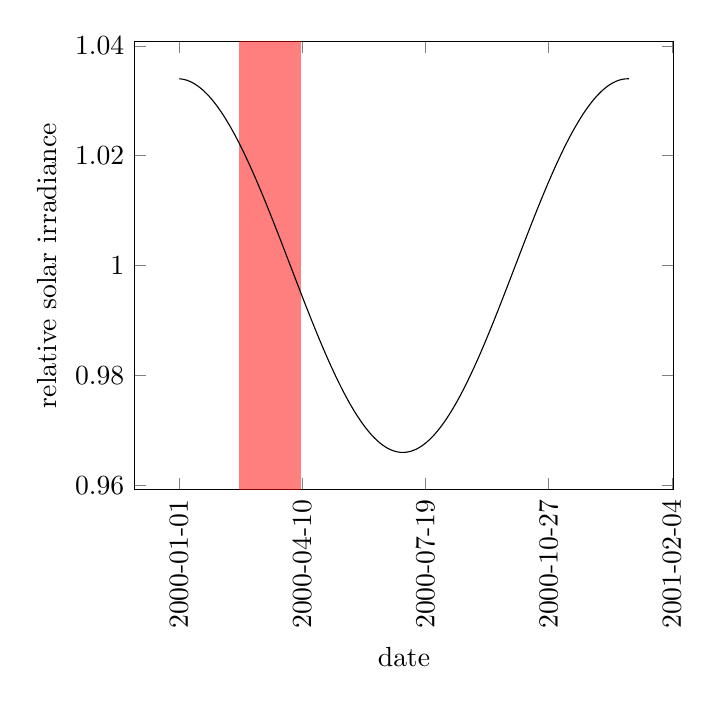
\begin{tikzpicture}
\begin{axis}[date coordinates in={x}, x tick label style={{rotate=90}}, xlabel={date}, ylabel={relative solar irradiance}]
    \draw[draw={none}, fill={red}, opacity={0.5}] ({axis cs:2000-02-19,0}|-{rel axis cs:0,1}) rectangle ({axis cs:2000-04-09,0}|-{rel axis cs:0,0});
    \addplot[no marks]
        table[row sep={\\}]
        {
            \\
            2000-01-01  1.0339949694264963  \\
            2000-01-02  1.0339798791946129  \\
            2000-01-03  1.033954733769792  \\
            2000-01-04  1.0339195405929695  \\
            2000-01-05  1.0338743100783727  \\
            2000-01-06  1.0338190556104383  \\
            2000-01-07  1.0337537935398526  \\
            2000-01-08  1.0336785431787123  \\
            2000-01-09  1.0335933267948096  \\
            2000-01-10  1.0334981696050436  \\
            2000-01-11  1.0333930997679577  \\
            2000-01-12  1.0332781483754074  \\
            2000-01-13  1.0331533494433587  \\
            2000-01-14  1.0330187399018236  \\
            2000-01-15  1.0328743595839311  \\
            2000-01-16  1.0327202512141402  \\
            2000-01-17  1.0325564603955968  \\
            2000-01-18  1.0323830355966392  \\
            2000-01-19  1.0322000281364558  \\
            2000-01-20  1.032007492169898  \\
            2000-01-21  1.0318054846714562  \\
            2000-01-22  1.031594065418399  \\
            2000-01-23  1.0313732969730849  \\
            2000-01-24  1.0311432446644486  \\
            2000-01-25  1.0309039765686694  \\
            2000-01-26  1.0306555634890264  \\
            2000-01-27  1.0303980789349465  \\
            2000-01-28  1.0301315991002518  \\
            2000-01-29  1.0298562028406122  \\
            2000-01-30  1.0295719716502123  \\
            2000-01-31  1.0292789896376335  \\
            2000-02-01  1.0289773435009675  \\
            2000-02-02  1.0286671225021589  \\
            2000-02-03  1.0283484184405922  \\
            2000-02-04  1.0280213256259267  \\
            2000-02-05  1.0276859408501886  \\
            2000-02-06  1.0273423633591292  \\
            2000-02-07  1.0269906948228555  \\
            2000-02-08  1.0266310393057452  \\
            2000-02-09  1.026263503235652  \\
            2000-02-10  1.0258881953724122  \\
            2000-02-11  1.0255052267756608  \\
            2000-02-12  1.0251147107719667  \\
            2000-02-13  1.0247167629212985  \\
            2000-02-14  1.0243115009828274  \\
            2000-02-15  1.0238990448800809  \\
            2000-02-16  1.0234795166654558  \\
            2000-02-17  1.0230530404841003  \\
            2000-02-18  1.0226197425371777  \\
            2000-02-19  1.0221797510445219  \\
            2000-02-20  1.021733196206694  \\
            2000-02-21  1.021280210166455  \\
            2000-02-22  1.0208209269696622  \\
            2000-02-23  1.0203554825256025  \\
            2000-02-24  1.0198840145667754  \\
            2000-02-25  1.0194066626081346  \\
            2000-02-26  1.0189235679058053  \\
            2000-02-27  1.0184348734152815  \\
            2000-02-28  1.0179407237491256  \\
            2000-02-29  1.0174412651341738  \\
            2000-03-01  1.0169366453682658  \\
            2000-03-02  1.016427013776509  \\
            2000-03-03  1.0159125211670903  \\
            2000-03-04  1.0153933197866507  \\
            2000-03-05  1.0148695632752314  \\
            2000-03-06  1.0143414066208105  \\
            2000-03-07  1.0138090061134397  \\
            2000-03-08  1.0132725192989942  \\
            2000-03-09  1.012732104932554  \\
            2000-03-10  1.0121879229314243  \\
            2000-03-11  1.0116401343278145  \\
            2000-03-12  1.0110889012211852  \\
            2000-03-13  1.0105343867302814  \\
            2000-03-14  1.009976754944862  \\
            2000-03-15  1.0094161708771439  \\
            2000-03-16  1.0088528004129715  \\
            2000-03-17  1.0082868102627291  \\
            2000-03-18  1.0077183679120083  \\
            2000-03-19  1.0071476415720455  \\
            2000-03-20  1.006574800129947  \\
            2000-03-21  1.0060000130987117  \\
            2000-03-22  1.0054234505670696  \\
            2000-03-23  1.00484528314915  \\
            2000-03-24  1.004265681933993  \\
            2000-03-25  1.0036848184349239  \\
            2000-03-26  1.0031028645387967  \\
            2000-03-27  1.002519992455132  \\
            2000-03-28  1.0019363746651573  \\
            2000-03-29  1.001352183870766  \\
            2000-03-30  1.0007675929434126  \\
            2000-03-31  1.000182774872958  \\
            2000-04-01  0.9995979027164776  \\
            2000-04-02  0.9990131495470529  \\
            2000-04-03  0.9984286884025539  \\
            2000-04-04  0.9978446922344366  \\
            2000-04-05  0.9972613338565628  \\
            2000-04-06  0.9966787858940617  \\
            2000-04-07  0.9960972207322477  \\
            2000-04-08  0.9955168104656087  \\
            2000-04-09  0.9949377268468805  \\
            2000-04-10  0.9943601412362225  \\
            2000-04-11  0.9937842245505093  \\
            2000-04-12  0.9932101472127538  \\
            2000-04-13  0.9926380791016763  \\
            2000-04-14  0.9920681895014345  \\
            2000-04-15  0.9915006470515298  \\
            2000-04-16  0.990935619696904  \\
            2000-04-17  0.9903732746382418  \\
            2000-04-18  0.9898137782824932  \\
            2000-04-19  0.9892572961936313  \\
            2000-04-20  0.9887039930436593  \\
            2000-04-21  0.9881540325638809  \\
            2000-04-22  0.9876075774964501  \\
            2000-04-23  0.987064789546213  \\
            2000-04-24  0.9865258293328568  \\
            2000-04-25  0.9859908563433795  \\
            2000-04-26  0.9854600288848957  \\
            2000-04-27  0.9849335040377905  \\
            2000-04-28  0.984411437609237  \\
            2000-04-29  0.9838939840870908  \\
            2000-04-30  0.9833812965941743  \\
            2000-05-01  0.9828735268429647  \\
            2000-05-02  0.9823708250907006  \\
            2000-05-03  0.9818733400949184  \\
            2000-05-04  0.9813812190694321  \\
            2000-05-05  0.9808946076407705  \\
            2000-05-06  0.9804136498050843  \\
            2000-05-07  0.9799384878855346  \\
            2000-05-08  0.9794692624901785  \\
            2000-05-09  0.9790061124703593  \\
            2000-05-10  0.9785491748796192  \\
            2000-05-11  0.9780985849331428  \\
            2000-05-12  0.9776544759677447  \\
            2000-05-13  0.9772169794024126  \\
            2000-05-14  0.9767862246994189  \\
            2000-05-15  0.9763623393260104  \\
            2000-05-16  0.9759454487166886  \\
            2000-05-17  0.9755356762360922  \\
            2000-05-18  0.9751331431424906  \\
            2000-05-19  0.9747379685519023  \\
            2000-05-20  0.9743502694028466  \\
            2000-05-21  0.973970160421739  \\
            2000-05-22  0.9735977540889426  \\
            2000-05-23  0.9732331606054825  \\
            2000-05-24  0.9728764878604362  \\
            2000-05-25  0.9725278413990074  \\
            2000-05-26  0.9721873243912932  \\
            2000-05-27  0.9718550376017545  \\
            2000-05-28  0.9715310793593984  \\
            2000-05-29  0.9712155455286807  \\
            2000-05-30  0.9709085294811384  \\
            2000-05-31  0.9706101220677594  \\
            2000-06-01  0.9703204115920983  \\
            2000-06-02  0.9700394837841456  \\
            2000-06-03  0.9697674217749596  \\
            2000-06-04  0.9695043060720657  \\
            2000-06-05  0.9692502145356338  \\
            2000-06-06  0.9690052223554372  \\
            2000-06-07  0.9687694020286036  \\
            2000-06-08  0.9685428233381619  \\
            2000-06-09  0.9683255533323916  \\
            2000-06-10  0.968117656304983  \\
            2000-06-11  0.9679191937760115  \\
            2000-06-12  0.9677302244737322  \\
            2000-06-13  0.9675508043172019  \\
            2000-06-14  0.9673809863997315  \\
            2000-06-15  0.9672208209731749  \\
            2000-06-16  0.9670703554330585  \\
            2000-06-17  0.9669296343045566  \\
            2000-06-18  0.9667986992293149  \\
            2000-06-19  0.9666775889531289  \\
            2000-06-20  0.9665663393144778  \\
            2000-06-21  0.9664649832339193  \\
            2000-06-22  0.9663735507043484  \\
            2000-06-23  0.9662920687821217  \\
            2000-06-24  0.9662205615790508  \\
            2000-06-25  0.9661590502552675  \\
            2000-06-26  0.9661075530129624  \\
            2000-06-27  0.9660660850909976  \\
            2000-06-28  0.9660346587603986  \\
            2000-06-29  0.9660132833207222  \\
            2000-06-30  0.966001965097305  \\
            2000-07-01  0.9660007074393911  \\
            2000-07-02  0.9660095107191421  \\
            2000-07-03  0.9660283723315256  \\
            2000-07-04  0.9660572866950872  \\
            2000-07-05  0.9660962452536014  \\
            2000-07-06  0.9661452364786041  \\
            2000-07-07  0.9662042458728034  \\
            2000-07-08  0.9662732559743704  \\
            2000-07-09  0.9663522463621058  \\
            2000-07-10  0.966441193661483  \\
            2000-07-11  0.9665400715515648  \\
            2000-07-12  0.9666488507727932  \\
            2000-07-13  0.9667674991356462  \\
            2000-07-14  0.9668959815301645  \\
            2000-07-15  0.9670342599363405  \\
            2000-07-16  0.9671822934353691  \\
            2000-07-17  0.9673400382217564  \\
            2000-07-18  0.967507447616282  \\
            2000-07-19  0.9676844720798129  \\
            2000-07-20  0.9678710592279622  \\
            2000-07-21  0.9680671538465909  \\
            2000-07-22  0.9682726979081465  \\
            2000-07-23  0.9684876305888344  \\
            2000-07-24  0.9687118882866161  \\
            2000-07-25  0.9689454046400313  \\
            2000-07-26  0.9691881105478338  \\
            2000-07-27  0.9694399341894409  \\
            2000-07-28  0.9697008010461855  \\
            2000-07-29  0.9699706339233678  \\
            2000-07-30  0.9702493529730981  \\
            2000-07-31  0.9705368757179257  \\
            2000-08-01  0.9708331170752443  \\
            2000-08-02  0.9711379893824705  \\
            2000-08-03  0.9714514024229834  \\
            2000-08-04  0.9717732634528222  \\
            2000-08-05  0.9721034772281298  \\
            2000-08-06  0.9724419460333376  \\
            2000-08-07  0.9727885697100805  \\
            2000-08-08  0.973143245686836  \\
            2000-08-09  0.9735058690092764  \\
            2000-08-10  0.9738763323713265  \\
            2000-08-11  0.9742545261469173  \\
            2000-08-12  0.9746403384224261  \\
            2000-08-13  0.9750336550297936  \\
            2000-08-14  0.9754343595803074  \\
            2000-08-15  0.9758423334990447  \\
            2000-08-16  0.9762574560599591  \\
            2000-08-17  0.9766796044216061  \\
            2000-08-18  0.9771086536634938  \\
            2000-08-19  0.9775444768230488  \\
            2000-08-20  0.9779869449331866  \\
            2000-08-21  0.9784359270604746  \\
            2000-08-22  0.978891290343878  \\
            2000-08-23  0.9793529000340752  \\
            2000-08-24  0.9798206195333321  \\
            2000-08-25  0.9802943104359242  \\
            2000-08-26  0.9807738325690922  \\
            2000-08-27  0.9812590440345225  \\
            2000-08-28  0.9817498012503358  \\
            2000-08-29  0.9822459589935767  \\
            2000-08-30  0.9827473704431864  \\
            2000-08-31  0.9832538872234501  \\
            2000-09-01  0.9837653594479034  \\
            2000-09-02  0.9842816357636864  \\
            2000-09-03  0.9848025633963311  \\
            2000-09-04  0.98532798819497  \\
            2000-09-05  0.985857754677952  \\
            2000-09-06  0.9863917060788516  \\
            2000-09-07  0.9869296843928589  \\
            2000-09-08  0.9874715304235355  \\
            2000-09-09  0.9880170838299235  \\
            2000-09-10  0.9885661831739928  \\
            2000-09-11  0.9891186659684134  \\
            2000-09-12  0.9896743687246377  \\
            2000-09-13  0.9902331270012797  \\
            2000-09-14  0.990794775452776  \\
            2000-09-15  0.9913591478783137  \\
            2000-09-16  0.9919260772710121  \\
            2000-09-17  0.9924953958673429  \\
            2000-09-18  0.9930669351967741  \\
            2000-09-19  0.9936405261316228  \\
            2000-09-20  0.9942159989371033  \\
            2000-09-21  0.994793183321554  \\
            2000-09-22  0.9953719084868293  \\
            2000-09-23  0.9959520031788422  \\
            2000-09-24  0.9965332957382407  \\
            2000-09-25  0.997115614151204  \\
            2000-09-26  0.9976987861003452  \\
            2000-09-27  0.9982826390157025  \\
            2000-09-28  0.9988670001258045  \\
            2000-09-29  0.9994516965087976  \\
            2000-09-30  1.0000365551436152  \\
            2000-10-01  1.0006214029611775  \\
            2000-10-02  1.0012060668956062  \\
            2000-10-03  1.0017903739354368  \\
            2000-10-04  1.0023741511748157  \\
            2000-10-05  1.0029572258646653  \\
            2000-10-06  1.0035394254638046  \\
            2000-10-07  1.004120577690005  \\
            2000-10-08  1.0047005105709734  \\
            2000-10-09  1.0052790524952397  \\
            2000-10-10  1.0058560322629413  \\
            2000-10-11  1.0064312791364813  \\
            2000-10-12  1.0070046228910559  \\
            2000-10-13  1.0075758938650232  \\
            2000-10-14  1.0081449230101116  \\
            2000-10-15  1.0087115419414419  \\
            2000-10-16  1.0092755829873568  \\
            2000-10-17  1.0098368792390358  \\
            2000-10-18  1.0103952645998877  \\
            2000-10-19  1.0109505738347009  \\
            2000-10-20  1.0115026426185385  \\
            2000-10-21  1.0120513075853657  \\
            2000-10-22  1.0125964063763913  \\
            2000-10-23  1.0131377776881134  \\
            2000-10-24  1.0136752613200513  \\
            2000-10-25  1.0142086982221508  \\
            2000-10-26  1.0147379305418502  \\
            2000-10-27  1.0152628016707919  \\
            2000-10-28  1.0157831562911643  \\
            2000-10-29  1.0162988404216635  \\
            2000-10-30  1.016809701463059  \\
            2000-10-31  1.0173155882433493  \\
            2000-11-01  1.0178163510624976  \\
            2000-11-02  1.0183118417367287  \\
            2000-11-03  1.018801913642381  \\
            2000-11-04  1.0192864217592925  \\
            2000-11-05  1.019765222713717  \\
            2000-11-06  1.0202381748207485  \\
            2000-11-07  1.0207051381262497  \\
            2000-11-08  1.0211659744482655  \\
            2000-11-09  1.0216205474179145  \\
            2000-11-10  1.0220687225197413  \\
            2000-11-11  1.022510367131523  \\
            2000-11-12  1.0229453505635133  \\
            2000-11-13  1.0233735440971168  \\
            2000-11-14  1.023794821022978  \\
            2000-11-15  1.0242090566784763  \\
            2000-11-16  1.0246161284846171  \\
            2000-11-17  1.0250159159823042  \\
            2000-11-18  1.0254083008679846  \\
            2000-11-19  1.025793167028658  \\
            2000-11-20  1.0261704005762353  \\
            2000-11-21  1.026539889881241  \\
            2000-11-22  1.026901525605845  \\
            2000-11-23  1.0272552007362183  \\
            2000-11-24  1.0276008106141996  \\
            2000-11-25  1.0279382529682661  \\
            2000-11-26  1.0282674279437958  \\
            2000-11-27  1.028588238132618  \\
            2000-11-28  1.0289005886018359  \\
            2000-11-29  1.029204386921921  \\
            2000-11-30  1.0294995431940623  \\
            2000-12-01  1.0297859700767706  \\
            2000-12-02  1.0300635828117228  \\
            2000-12-03  1.0303322992488448  \\
            2000-12-04  1.0305920398706192  \\
            2000-12-05  1.0308427278156171  \\
            2000-12-06  1.0310842889012428  \\
            2000-12-07  1.0313166516456844  \\
            2000-12-08  1.0315397472890675  \\
            2000-12-09  1.0317535098138022  \\
            2000-12-10  1.0319578759641181  \\
            2000-12-11  1.0321527852647834  \\
            2000-12-12  1.0323381800390001  \\
            2000-12-13  1.0325140054254722  \\
            2000-12-14  1.0326802093946388  \\
            2000-12-15  1.0328367427640717  \\
            2000-12-16  1.032983559213028  \\
            2000-12-17  1.033120615296159  \\
            2000-12-18  1.0332478704563641  \\
            2000-12-19  1.0333652870367946  \\
            2000-12-20  1.0334728302919949  \\
            2000-12-21  1.033570468398186  \\
            2000-12-22  1.0336581724626808  \\
            2000-12-23  1.0337359165324362  \\
            2000-12-24  1.033803677601731  \\
            2000-12-25  1.0338614356189744  \\
            2000-12-26  1.0339091734926402  \\
            2000-12-27  1.0339468770963234  \\
            2000-12-28  1.0339745352729208  \\
            2000-12-29  1.0339921398379335  \\
            2000-12-30  1.0339996855818872  \\
            2000-12-31  1.0339971702718747  \\
        }
        ;
\end{axis}
\end{tikzpicture}
\end{document}
